\documentclass[11pt]{article}

\usepackage{amsmath, amssymb}
\usepackage{graphicx}
\usepackage{xcolor}
\usepackage{booktabs}
\usepackage{geometry}
\usepackage{booktabs,longtable,array}
\usepackage{tabularx}
\usepackage[
  backend=biber,
  style=numeric-comp,
  sorting=none,
  maxbibnames=5,
  minbibnames=5,
  giveninits=true,
  doi=false, isbn=false, url=false, eprint=false
]{biblatex}
\addbibresource{references.bib}
\usepackage[hidelinks]{hyperref}

\geometry{margin=1in} 

\title{Modelling mass TB and TBI screening in South Tarawa (Kiribati) --- Methods appendix}
\date{}
\author{Romain Ragonnet}

\begin{document}
 
\maketitle

\tableofcontents
\clearpage

%%%%%%%%%%%%%%%%%%%%%%%%%%%%%%%%%%%%%%%%%%%%%%%%%%%%%%%%%%%%
\section{Overview of the Model and Analysis}

We developed a deterministic, age-structured compartmental model of \textit{Mycobacterium tuberculosis} (M.tb) transmission, infection, tuberculosis (TB) disease, detection, treatment, and prevention. The model uses discrete age groups and continuous time, and is formulated as a system of ordinary differential equations (ODEs). All compartments are stratified by age group and by screening reachability, so that each model state is indexed by both dimensions.

\paragraph{Compartment notation (per age group and reachability stratum).}
We denote the following compartments:
\begin{itemize}
    \item \(\mathbf{S}\): M.tb-\emph{na\"ive} (never infected).
    \item \(\mathbf{E}\): Incipient infection (post-infection with risk of disease progression).
    \item \(\mathbf{C}\): Contained infection (immune control without sterilisation - no immediate disease progression risk).
    \item \(\mathbf{X}\): Cleared infection (post infection clearance - spontaneous or induced by tuberculosis preventive treatment, TPT).
    \item \(\mathbf{D_{AL}}\): Active TB, \underline{A}symptomatic, \underline{L}ow infectiousness.
    \item \(\mathbf{D_{SL}}\): Active TB, \underline{S}ymptomatic, \underline{L}ow infectiousness.
    \item \(\mathbf{D_{AH}}\): Active TB, \underline{A}symptomatic, \underline{H}igh infectiousness.
    \item \(\mathbf{D_{SH}}\): Active TB, \underline{S}ymptomatic, \underline{H}igh infectiousness.
    \item \(\mathbf{T}\): On TB treatment.
    \item \(\mathbf{R}\): Recovered (post self-recovery or treatment).
\end{itemize}

\noindent We use the term ``M.tb na\"ive'' rather than the commonly used ``Susceptible'' to describe individuals who have never been infected with M.tb, because several non-na\"ive compartments remain (partially) susceptible to reinfection.

\paragraph{Model structure.}
Figure~\ref{fig:model-structure} shows the model compartments and the transitions between them.
\begin{figure}[!ht]
\centering
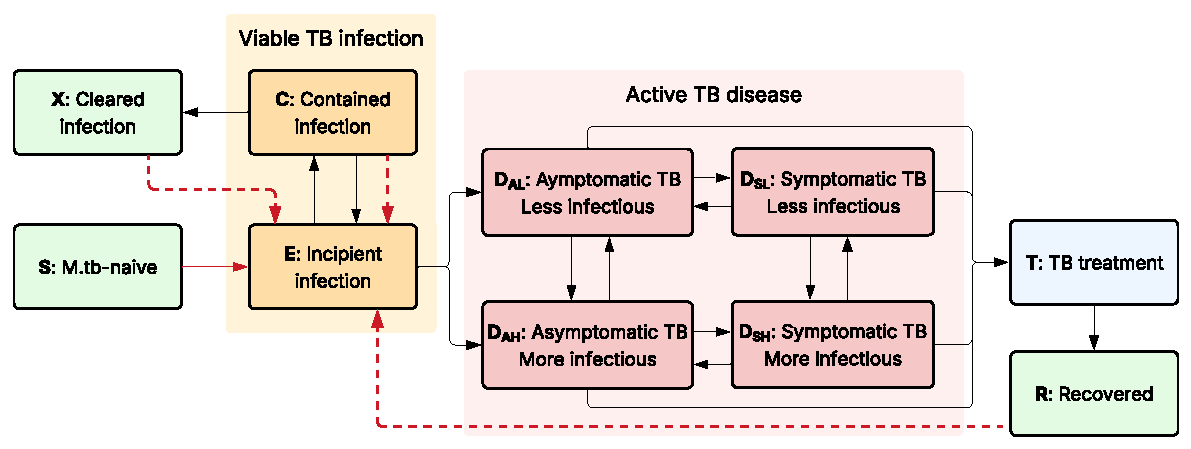
\includegraphics[width=\textwidth]{figures/tb_model.pdf}
\caption{\textbf{Schematic of model compartments and transitions.}
Transmission pathways are shown in red, with dashed red arrows indicating reinfection. For clarity, age and screening-reachability stratification, births, natural mortality, spontaneous recovery from asymptomatic TB, and TB-related mortality from symptomatic TB are not shown.
}
\label{fig:model-structure}
\end{figure}

\paragraph{Model overview.}
Non-disease M.tb infection is modelled through two stages: incipient (\(E\)) and contained (\(C\)). 
The contained stage represents a state in which the infection is controlled by the immune system, with no immediate risk of progression to active disease. 
Breakdown of containment reflects loss of immune control, returning individuals to the incipient stage (\(E\)) with a renewed risk of disease progression. 
Containment can also result in complete clearance of infection, represented by state \(X\).

Progression from \(E\) results in asymptomatic active disease (more or less infectious) that may gain/lose infectiousness and progress/regress between symptomatic and asymptomatic states. More details about the disease categorisation and transitions are provided in Section~\ref{sec:tb_disease}. 
Only \emph{symptomatic} forms of disease are detected through passive case finding; while active screening may potentially detect any form of TB. Screening programmes add time-limited detection flows for both TB disease and non-disease M.tb infection states (Section~\ref{sec:screening}).

Age-specific demography and mixing are implemented explicitly to capture the effects of population structure and contact patterns on transmission dynamics (Sections~\ref{sec:demog}--\ref{sec:mixing-matrix}).

The model is additionally stratified by screening reachability, distinguishing individuals who can participate in active screening from those who are hard to reach. The latter receive no active screening and are assumed to have greater susceptibility to infection and poorer access to passive case detection (Section~\ref{sec:reachability}).

\paragraph{Simulation period and initial conditions.}
The model is simulated from 1850 to 2035. The initial population size is set to the earliest available estimate for the modelled population (1950) from the United Nations World Population Prospects (WPP), and no population growth is applied before that first data year, so the population size remains constant over the initial period and follows the observed trajectory thereafter (Section~\ref{sec:demog}).
The epidemic is seeded at the start of the simulation with 100 individuals in the symptomatic, high-infectiousness disease state (\(D_{SH}\)), with the remainder of the population placed in the M.tb-na\"ive compartment (\(S\)).
The long period preceding the first calibration data allows the age distribution and the TB epidemic to reach an endemic equilibrium well before the period informed by observations, so that results are insensitive to the size and composition of the initial seed.

\paragraph{Parameter treatment in calibration.}
Parameters with specified prior distributions are estimated in the Bayesian calibration while those without priors are fixed. 
Estimated classes include core transmission (baseline transmission rate and population-scaling exponent), social mixing (background mixing level, age assortativity spread, and parent–child mixing strength), selected early-infection and disease-transition rates (clearance, immunity breakdown, progression to symptomatic disease, gain of infectiousness), the passive-detection scale-up profile, and a subset of diagnostic sensitivities. 

\paragraph{Model use in analysis.}
The model is used in two stages: (i) to reconstruct the historical epidemic trajectory by calibrating uncertain parameters to epidemiological and intervention data; and (ii) to project forward under alternative intervention scenarios (screening and preventive treatment). Parameter estimation is performed in a Bayesian framework with Differential Evolution Metropolis algorithm (DEMetropolisZ); posterior samples are propagated to quantify uncertainty in projected outcomes.
Two influential quantities that the data cannot identify are handled by repeating the whole analysis across a grid of fixed values, giving sixteen independently calibrated model configurations, and three further sensitivity analyses vary a single assumption each (Section~\ref{sec:configs}).

%%%%%%%%%%%%%%%%%%%%%%%%%%%%%%%%%%%%%%%%%%%%%%%%%%%%%%%%%%%%
\section{Software and Code}

The model is implemented in Python using \texttt{summer2}, a domain-specific language for compartmental epidemiological models. Models are declared in terms of compartments, the flows between them, and stratifications applied to existing structure, so that the code corresponds closely to the epidemiological assumptions it encodes and can be read and checked without reference to the numerical implementation.

Simulations are accelerated using \texttt{jax} just-in-time compilation, which compiles the model to optimised machine code on first execution; subsequent simulations require \(\sim\)200\,ms each, which makes calibration at the scale described in Section~\ref{sec:calibration-algorithm} tractable. The acceleration is obtained through compilation alone: no machine-learning surrogate, emulator or other approximation of the model is involved, and the compiled model is numerically equivalent to the uncompiled one.

Bayesian calibration is performed using \texttt{estival}, a companion package that connects a \texttt{summer2} model to the samplers provided by \texttt{PyMC}, handling the specification of priors, calibration targets and likelihood. The same model object is used for calibration and for scenario projection.

The same software stack has been used in previously published modelling analyses across a range of pathogens and settings, including analyses of school closures and COVID-19 dynamics across 74 countries~\cite{ragonnet2025}, of the effect of pandemic-related disruptions on TB in Vietnam~\cite{bui2025}, and of Australia's 2022 Omicron waves~\cite{trauer2025}.

All model code, calibration routines, analysis scripts, and interactive notebooks are available at \url{https://github.com/monash-emu/kiribati_tb_modelling}.

The repository includes instructions for installation and reproduction of results. The project environment is managed using \texttt{pixi} for reproducible dependency management and straightforward installation.

%%%%%%%%%%%%%%%%%%%%%%%%%%%%%%%%%%%%%%%%%%%%%%%%%%%%%%%%%%%%
\section{Population Structure and Demography}
\label{sec:demog}

The population is stratified by age, and every age and disease state in the model is subject to the appropriate all‑cause and TB‑specific mortality rates. Age‑specific all-cause (non-TB) mortality rates and the total population size over time are taken from the WPP, as described in Section~\ref{sec:demog-inputs}.

Rather than specifying a birth rate independently, the model reproduces the observed population trajectory by construction, through two devices.

First, every death is implemented as a \emph{transition} into the youngest M.tb-na\"ive compartment, rather than as an exit from the model. This applies to all-cause deaths from every compartment and age group, to TB deaths from the symptomatic disease states, and to deaths occurring on treatment. Each death therefore removes an individual from their current state and simultaneously returns a newborn, so that mortality redistributes the population across ages and states without altering its total size.

Second, an additional entry flow \(\mathcal{B}(t)\) is directed into that same youngest M.tb-na\"ive compartment to generate population growth. Its magnitude is the year-on-year increment of the observed total population series, interpolated to give a smooth function of time and set to zero before the first data year, so that the population remains constant over the period preceding the data.

Taken together, the two devices are equivalent to setting the birth flow equal to the number of deaths plus the observed net increase in population size. Because deaths are the only outflow and are fully recycled, the modelled total population \(N(t)\) satisfies
\[
\frac{dN}{dt} = \mathcal{B}(t),
\]
so that \(N(t)\) follows the observed trajectory exactly, while its distribution across age groups and across infection and disease states is determined by the model's internal dynamics. Note that fertility data are not used to generate births; they enter the model only through the parent--child component of the mixing matrix (Section~\ref{sec:mixing-matrix}).

Ageing is implemented as first-order transitions between adjacent age groups, with rates calculated as the inverse of the age group's span and applied to all age strata except the oldest one.
%%%%%%%%%%%%%%%%%%%%%%%%%%%%%%%%%%%%%%%%%%%%%%%%%%%%%%%%%%%%
\subsection{Age Groups and Ageing}

\paragraph{Age groups.}
The population is stratified into \(G = 8\) age groups with lower bounds
\[
\mathcal{A} = \{0, 3, 5, 10, 15, 18, 40, 65\}.
\]
The final group is open-ended (65+).

The breaks were chosen so that every age-dependent process and observation used in the analysis aligns exactly with a group boundary, avoiding the need to apportion parameters or targets within groups:

\begin{itemize}
\item \textbf{3 years} is the minimum age of eligibility for screening under the PEARL algorithm, below which no active screening or preventive treatment is offered.
\item \textbf{5 and 15 years} delimit the three age categories used for the early-infection parameters (\(<5\), 5--14, 15+), and 15 years additionally separates the age groups in which susceptibility to infection is reduced to reflect protection from bacille Calmette--Gu\'erin (BCG) vaccination and infectiousness is set to zero.
\item \textbf{10 years} separates children receiving symptom screening only from older individuals additionally receiving chest X-ray and, in the PEARL algorithm, frontline Xpert.
\item \textbf{18 years} allows the model to reproduce the earlier estimate of tuberculin skin test (TST) positivity among adults aged 18 years and over, which is used as a calibration target (Section~\ref{sec:calib-data}).
\item \textbf{40 and 65 years} subdivide the adult population to capture differences in background mortality and in contact patterns across adult ages.
\end{itemize}

%%%%%%%%%%%%%%%%%%%%%%%%%%%%%%%%%%%%%%%%%%%%%%%%%%%%%%%%%%%%
\subsection{Age-Mixing Matrix}
\label{sec:mixing-matrix}

\paragraph{Notation and data sources.}
Let \(i,j \in \{1,\dots,G\}\) index age groups and \([a_i,b_i]\) denote the single ages in group \(i\). Calendar time is \(t\) (years). 
The construction uses the WPP population and fertility series described in Section~\ref{sec:demog-inputs}; for modelled years outside the data ranges, quantities are clamped to the nearest available year.
\paragraph{Overview.}
At time \(t\), we construct an age-specific contact matrix
\[
\mathbf{C}(t) = \big(C_{ij}(t)\big)_{i,j=1}^G,
\]
where \(C_{ij}(t)\) is the per-capita rate at which age group \(i\) contacts age group \(j\). Construction proceeds by:
(1) building a symmetric per-pair intensity matrix \(\mathbf{S}(t)\);
(2) scaling columns by the contacted group size;
(3) normalising by the spectral radius.
We combine three components: uniform background mixing, assortative age mixing, and parent–child mixing. Three scalar parameters govern these components (background level, assortativity spread, and parent–child mixing strength) and are estimated.

\paragraph{Population weights within age groups.}
To allow non-uniform single-age distributions within groups, let \(N(a,t)\) be the population at age \(a\) and time \(t\). For group \(i\),
\[
w_i(a,t) = \frac{N(a,t)}{\sum_{a' \in [a_i,b_i]} N(a',t)},\qquad
\sum_{a \in [a_i,b_i]} w_i(a,t)=1.
\]

\paragraph{Symmetric per-pair intensity.}
For each \(i,j\),
\[
S_{ij}(t) = b + S^{\mathrm{assort}}_{ij}(t) + \kappa_{\mathrm{pc}}\, S^{\mathrm{pc}}_{ij}(t),
\quad S_{ij}(t)=S_{ji}(t),
\]
where \(b\) is the background level (\texttt{bg\_mixing}), \(S^{\mathrm{assort}}\) is an exponential kernel with spread \(\ell\) (\texttt{a\_spread}), and \(S^{\mathrm{pc}}\) encodes parent–child contacts from fertility patterns, with strength \(\kappa_{\mathrm{pc}}\) (\texttt{pc\_strength}). Smaller values of \(\ell\) correspond to more strongly assortative mixing by age.

\emph{Assortative age mixing.}
\[
S^{\mathrm{assort}}_{ij}(t)
=
\sum_{a \in [a_i,b_i]}
\sum_{c \in [a_j,b_j]}
w_i(a,t)\, w_j(c,t)\,
\frac{1}{\ell}
\exp\!\left(-\frac{|a-c|}{\ell}\right).
\]

\emph{Parent–child mixing.}
Let \(p_{\mathrm{pc}}(\Delta, y)\) be the probability of a parent–child age gap \(\Delta\) for a child born in year \(y\). With \(a_{\mathrm{child}}=\min(a,c)\) and birth year \(t-a_{\mathrm{child}}\),
\[
S^{\mathrm{pc}}_{ij}(t)
=
\sum_{a \in [a_i,b_i]}
\sum_{c \in [a_j,b_j]}
w_i(a,t)\, w_j(c,t)\,
p_{\mathrm{pc}}\!\left(|a-c|,\; t - a_{\mathrm{child}}\right).
\]

\paragraph{Population scaling and asymmetry.}
The per-pair matrix becomes an asymmetric WAIFW matrix by column scaling with the contacted group size:
\[
C_{ij}(t) = S_{ij}(t)\, N_j(t).
\]

\paragraph{Normalisation.}
Let \(\rho(t)\) be the spectral radius of \(\mathbf{C}(t)\). We use the normalised matrix
\[
\tilde{\mathbf{C}}(t) = \frac{\mathbf{C}(t)}{\rho(t)}.
\]

%%%%%%%%%%%%%%%%%%%%%%%%%%%%%%%%%%%%%%%%%%%%%%%%%%%%%%%%%%%%
\section{Natural History of Infection and Disease}
We represent early TB infection dynamics using two non-disease states: an \emph{incipient} state (E) and a \emph{contained} state (C). Individuals newly infected with M.tb enter E, where infection is unstable and at risk of progression. From E, they may either progress to asymptomatic active TB or undergo immune-mediated containment, moving to C. Contained infection may subsequently clear entirely to X (uninfected/cleared) or experience immunological failure, returning to the incipient state E.
Active TB is stratified by both symptom status (asymptomatic vs. symptomatic) and infectiousness (low vs. high), yielding four disease compartments: $D_{AL}, D_{SL}, D_{AH}, D_{SH}$. Individuals with asymptomatic disease may progress to symptomatic disease, and symptomatic disease may regress to asymptomatic; similarly, infectiousness may increase (low $\to$ high) or decrease (high $\to$ low).
However, transitions are restricted to a single dimension at a time. Individuals may change symptom status (asymptomatic $\leftrightarrow$ symptomatic) or infectiousness (low $\leftrightarrow$ high), but simultaneous transitions in both dimensions are not allowed. 
Self-recovery is allowed only from asymptomatic states, with recovered individuals entering $R$. In contrast, TB-induced mortality rates are only applied to the symptomatic states.
Treatment is available for all active states, with successful treatment leading to recovery ($R$) and unsuccessful treatment resulting in relapse to asymptomatic low infectiousness ($D_{AL}$) or death.

\paragraph{Early infection.}
Progression from \(E\) is age-specific (three categories: $<5$, 5--14, 15+) and partitioned into low vs high infectiousness at first presentation. In the absence of data informing this split, progression from incipient infection is divided equally between the less-infectious and the more-infectious asymptomatic states (\(p=0.5\)). This assumption is not restrictive, because the subsequent within-disease transition rates are estimated during calibration, so that the resulting distribution of prevalent TB across the four disease states reproduces the observed data regardless of the initial split. Containment rates are also age-specific. Clearance and immune breakdown are age-invariant.

\paragraph{Symptom status and infectiousness transitions.}
\label{sec:tb_disease}
Movements between asymptomatic and symptomatic states, and between low and high infectiousness, govern within-disease dynamics. The cross-sectional observations available from the completed PEARL screening phase constrain the relative sizes of the four disease compartments, but not the speed at which individuals move between them: the same distribution of prevalent TB across states can be reproduced by slow or by rapid transitions in both directions. To resolve this identifiability problem, the two regression rates (symptomatic \(\to\) asymptomatic and high \(\to\) low infectiousness) are fixed at a common value, while the two corresponding progression rates (asymptomatic \(\to\) symptomatic and low \(\to\) high infectiousness) are estimated during calibration. The value adopted for the regression rate, the priors placed on the estimated rates, and the range over which the regression rate is varied are given in Section~\ref{sec:params}.

\paragraph{Reinfection.}
Reinfection is permitted from \(C\), \(X\), and \(R\) with relative susceptibilities \(\rho_C\) (contained) and \(\rho_X=\rho_R\) (cleared and recovered), and a child susceptibility modifier \(\sigma^{\text{child}}\) applied when infection arises from \(S\) in $<15$\,y groups.
This adjustment captures the effect of BCG vaccination, which is typically administered in infancy and provides protection against infection for several years.

\paragraph{Infectiousness weighting.}
Let \(\sigma_A\) denote the relative infectiousness of asymptomatic vs symptomatic disease, and \(\sigma_L\) the relative infectiousness of low vs high. Define the active-disease index set
\[
\mathcal{K}=\{AL,SL,AH,SH\},
\]
with relative infectiousness weights \(w_k\) given by \(w_{SH}=1\), \(w_{SL}=\sigma_L\), \(w_{AH}=\sigma_A\), \(w_{AL}=\sigma_A\sigma_L\). Children under 15 years contribute zero infectiousness, implemented by setting \(w_k=0\) in those age groups.

%%%%%%%%%%%%%%%%%%%%%%%%%%%%%%%%%%%%%%%%%%%%%%%%%%%%%%%%%%%%
\section{Stratification by Screening Reachability}
\label{sec:reachability}

Population-wide screening never reaches the entire population, and the individuals who are not reached may differ epidemiologically from those who participate. To capture this, the model is stratified into two mutually exclusive strata: a \emph{screening-reachable} stratum, comprising individuals who can participate in active screening, and a \emph{hard-to-reach} stratum, comprising individuals who do not. This stratification is applied to all compartments and is crossed with the age stratification, so that each model state is indexed by both age group \(i\) and reachability stratum \(s \in \{\mathrm{r}, \mathrm{u}\}\).

\paragraph{Population split.}
The proportion of the population in the screening-reachable stratum is denoted \(\pi\) (Section~\ref{sec:params}). The initial population is split between the two strata according to \(\pi\) and \(1-\pi\) within every compartment and age group.

The stratum sizes are held at these proportions over time. Because there are no transitions between the screening-reachable and hard-to-reach strata, this is achieved by (i) splitting the additional births used to reproduce population growth between the two strata according to \(\pi\) and \(1-\pi\), and (ii) returning all deaths (background, TB-related, and on-treatment) to the M.tb-na\"ive compartment of the youngest age group \emph{within the same reachability stratum} from which they originated. Reachability is therefore a fixed, lifelong attribute in the model, and the fraction of the population that is hard to reach does not drift as the epidemic or the interventions evolve.
Mixing between the screening-reachable and hard-to-reach strata is assumed to be homogeneous. In the absence of data on the contact patterns of individuals not reached by screening, this is a deliberately conservative assumption: assortative mixing within the hard-to-reach stratum would be expected to further concentrate residual transmission in that group.

\paragraph{Epidemiological differences between strata.}
Barriers to participating in screening are unlikely to occur in isolation and may coincide with living conditions or health-seeking behaviours that also affect TB risk and access to routine diagnosis. Two multiplicative adjustments are therefore applied to the hard-to-reach stratum, relative to the screening-reachable stratum:

\begin{itemize}
    \item \textbf{Susceptibility to infection.} All infection and reinfection flows (from \(S\), \(C\), \(X\) and \(R\)) are multiplied by \(\theta_{\mathrm{sus}}\) (\texttt{rel\_sus\_unreachable}) in the hard-to-reach stratum, so that hard-to-reach individuals acquire infection at a higher rate than screening-reachable individuals experiencing the same force of infection. This factor is applied to the susceptibility side of transmission only; the relative infectiousness of individuals with TB does not differ by stratum.
    \item \textbf{Passive detection.} The time-varying passive detection rate \(\delta(t)\) (Section~\ref{sec:screening}) is multiplied by \(\theta_{\mathrm{det}}\) (\texttt{rel\_detection\_unreachable}) in the hard-to-reach stratum, reflecting an assumption of reduced access to routine diagnostic services in the same population that is difficult to reach through active screening.
\end{itemize}

\noindent Neither multiplier is informed by the available data, so both are fixed rather than estimated; their values, and the range over which \(\theta_{\mathrm{sus}}\) is varied, are given in Section~\ref{sec:params}.

\paragraph{Access to screening.}
All active screening flows, for both TB disease and non-disease M.tb infection, are set to zero in the hard-to-reach stratum. Screening programmes therefore act exclusively on the screening-reachable stratum, and the maximum achievable coverage of the total population is \(\pi\): a nominal coverage equal to \(\pi\) corresponds to screening essentially the whole screening-reachable stratum, whereas lower nominal coverage levels represent incomplete participation among screening-reachable individuals (Section~\ref{sec:screening}).

\paragraph{Calibration and reporting.}
Because the epidemiological observations collected during the completed PEARL screening phase were made among participants, the corresponding calibration targets (measured TB prevalence and TST positivity) are compared with model outputs restricted to the screening-reachable stratum. Historical notifications, which arise from passive detection in the whole population, are compared with model outputs aggregated across both strata. Projected burden outcomes are likewise reported for the entire modelled population unless otherwise stated, and the share of TB incidence arising from the hard-to-reach stratum is tracked as an additional output.

%%%%%%%%%%%%%%%%%%%%%%%%%%%%%%%%%%%%%%%%%%%%%%%%%%%%%%%%%%%%
\section{Transmission and Force of Infection}
\label{sec:transmission}

We interpolate between frequency- and density-dependent transmission using the exponent \(\kappa\in[0,1]\) applied to the contacted population size. Because mixing between reachability strata is homogeneous (Section~\ref{sec:reachability}), the force of infection depends on age group only. For age group \(i\) it is
\[
\lambda_i(t)
=
\beta_0\, N_{\mathrm{ref}}^{\,\kappa}
\sum_{j}
\tilde{C}_{ij}(t)\;
\frac{I^{\mathrm{eff}}_j(t)}{N_j(t)^{\kappa}},
\]
where \(\tilde{C}(t)\) is the spectral-radius-normalised age-mixing matrix (Section~\ref{sec:mixing-matrix}).  Here \(N_{\mathrm{ref}}\) denotes the total population in year 2020 and is included purely as a scaling constant for more efficient calibration. This rescaling stabilises the magnitude of the transmission coefficient \(\beta_0\) across different values of \(\kappa\), preventing its calibrated value from varying by orders of magnitude as the dependence on population size changes.
The effective infectious pool and the population size of age group \(j\) are both aggregated over the two reachability strata \(s\in\{\mathrm{r},\mathrm{u}\}\):
\[
I^{\mathrm{eff}}_j(t) =
\sum_{s}\ \sum_{k\in\mathcal{K}} w_k\, D_{k,j,s}(t),
\qquad
N_j(t) = \sum_{s} N_{j,s}(t).
\]
Infectiousness weights \(w_k\) do not differ by reachability stratum; only susceptibility does, through the multiplier \(\theta^{\mathrm{sus}}_s\) introduced in Section~\ref{sec:reachability}.

%%%%%%%%%%%%%%%%%%%%%%%%%%%%%%%%%%%%%%%%%%%%%%%%%%%%%%%%%%%%
\section{TB Detection, Treatment and Screening}
\label{sec:screening}

\subsection{Passive Detection}
Passive case finding applies \emph{only to symptomatic disease}. Asymptomatic disease does not, by definition, prompt care seeking, so that individuals with asymptomatic TB can enter treatment only after progressing to symptomatic disease, or through active screening.

The passive detection rate is allowed to vary over time, because diagnostic capacity and access to care in Kiribati have strengthened progressively over recent decades, and a constant rate would be difficult to reconcile with the historical notification series. Denote the time-varying passive detection profile by \(\delta(t)\), which follows a smooth hyperbolic-tangent scale-up from an earlier (lower) level to a recent level:
\[
\delta(t)
=
\delta_{\mathrm{rec}}
\Bigg[
\phi
+
(1-\phi)\,
\Bigg(
\frac{\tanh\!\big(\sigma\, (t - t^\ast)\big)}{2}
+
\frac{1}{2}
\Bigg)
\Bigg].
\]
Here, \(\delta_{\mathrm{rec}}\) is the recent detection level, \(\phi\in(0,1]\) is the past-to-recent ratio, \(\sigma>0\) controls steepness, and \(t^\ast\) is the inflection time.

Figure~\ref{detect} illustrates an example profile for 
$\delta_{\mathrm{rec}} = 0.7$, $\phi = 0.5$, $\sigma = 0.15$ and $t^\ast = 2005$.
\begin{figure}[!ht]
\centering
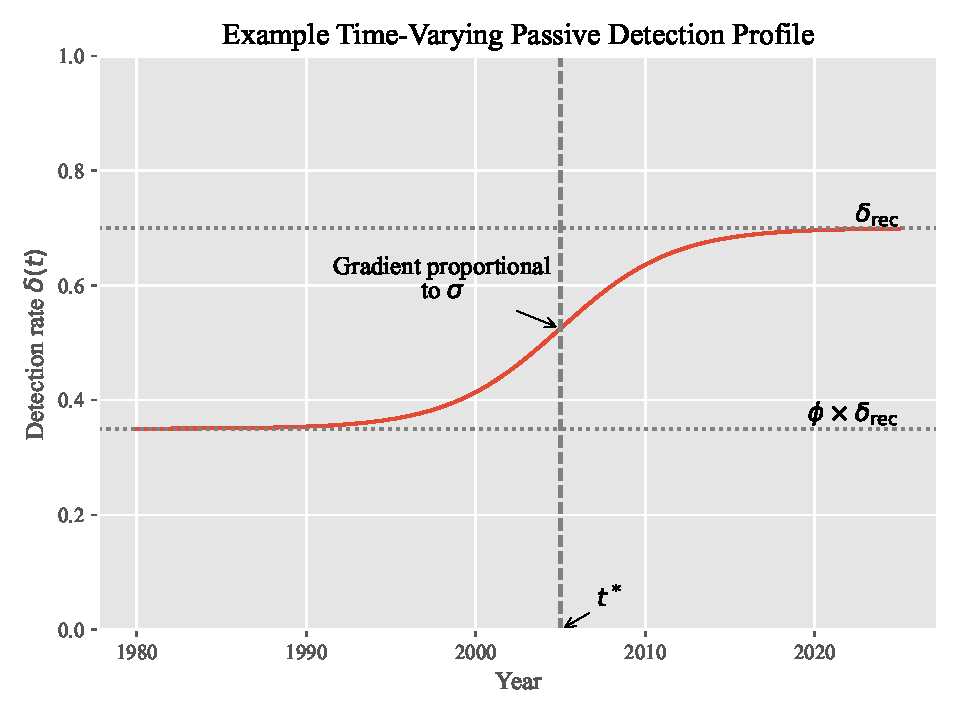
\includegraphics[width=0.6\textwidth]{figures/pdetection_profile.pdf}
\caption{Example time-varying passive detection profile for symptomatic TB disease.}   
\label{detect}
\end{figure}

\subsection{Treatment outcomes}
During treatment, individuals may experience three mutually exclusive outcomes: successful recovery, relapse, or death. Relapse here encompasses all unsuccessful outcomes other than death, including treatment failure and loss to follow-up; these individuals return to the asymptomatic, less-infectious disease state and remain subject to subsequent detection. Recovery occurs at a rate depending on the time-varying treatment success rate (TSR):
\[
\text{Recovery: } \quad \text{rate} = \frac{\text{TSR}(t)}{\tau},
\]
where \(\text{TSR}(t)\) denotes the proportion of successful treatments at time \(t\), and \(\tau\) is the average treatment duration.  

Age-specific relapse and treatment-death rates are calculated to account for both background mortality and the fixed proportion of treatment episodes that result in negative outcomes. Let \(\mu_i\) be the natural mortality rate for age group \(i\). The fixed fraction of negative outcomes resulting in death is denoted \(f_\text{neg}\).

The expected proportion of individuals dying from natural causes while on treatment is:
\[
p^{\text{nat\_death}}_i = 1 - e^{-\tau \mu_i}.
\]

The target proportion of deaths due to treatment failure (excluding natural mortality) is calculated as the fraction of negative outcomes allocated to death:
\[
p^{\text{tx\_death}} = (1 - \text{TSR}(t)) \cdot f_\text{neg}.
\]

To ensure that the overall probability of death on treatment remains non-negative after accounting for natural mortality, the treatment-death rate is defined as:
\[ 
\mu^{\text{TX}}_i = \frac{\max \{ p^{\text{tx\_death}} - p^{\text{nat\_death}}_i, 0 \}}{\tau}.
\]

Finally, the age-specific relapse rate is derived from the residual fraction of unsuccessful treatment episodes, after subtracting both treatment deaths and natural deaths:
\[
\phi_i = \frac{1 - \text{TSR}(t) - \tau \mu^{\text{TX}}_i - p^{\text{nat\_death}}_i}{\tau}.
\] 

These equations ensure that the sum of recovery, relapse, and treatment-death probabilities over the course of treatment equals one, while explicitly incorporating time-varying treatment success and age-specific background mortality.

\subsection{Screening programmes}

We consider a set of time-limited screening interventions implemented over the year 2026. Each programme is defined by three elements: the algorithm applied in each targeted age group, the age groups targeted, and the coverage achieved.

\paragraph{Coverage.}
Three coverage levels are explored: 65\%, 75\% and 85\%. These are expressed as proportions of the \emph{total} target population, that is, with hard-to-reach individuals included in the denominator, so that the highest level corresponds to essentially complete coverage of the screening-reachable stratum (Section~\ref{sec:reachability}). It is implemented as 84.5\%, because complete coverage of that stratum would require an infinite screening rate under the constant-hazard formulation used here.

Coverage is translated into a constant per-capita screening rate applied to the screening-reachable stratum over the intervention period. If \(c\) denotes the target coverage of the total population (expressed as a proportion), \(\pi\) the screening-reachable fraction, and \(\Delta t\) the duration of the campaign, the screening rate is
\[
r = -\frac{\log(1 - c/\pi)}{\Delta t},
\]
under which a proportion \(c/\pi\) of the eligible screening-reachable population, and hence a proportion \(c\) of the total target population, is screened over the campaign. The rate is implemented as a time-varying function that is zero outside the intervention window and constant during it. Age groups not targeted by a given programme are assigned a screening rate of zero, applied as a multiplicative coverage adjustment during age stratification.

\paragraph{Screening flows.}
Screening may act on active TB disease or on non-disease M.tb infection. Sensitivities in the model are properties of a complete \emph{algorithm} rather than of an individual test: we write \(s^{A}_k\) for the sensitivity of approach \(A\) in state \(k\), that is, the probability that a person occupying that state, and screened under that approach, is correctly identified and referred for treatment. An individual in state \(k\) therefore leaves it through screening at hazard \(s^{A}_k\, r\), which is the quantity denoted \(\zeta_{k,i}(t)\) in Section~\ref{sec:odes}. Individuals identified with TB disease are moved to the treatment compartment (\(T\)). Individuals identified as infected are offered TPT, and the hazard is further multiplied by the probability of completing it, so that only completers move to the cleared compartment (\(X\)).

\paragraph{Approaches to detecting TB disease.}
We consider three approaches, in increasing order of intensity:

\begin{itemize}
    \item \textbf{Symptom screening (SSx)}: screening on the basis of reported symptoms alone. Symptomatic disease is assumed to be identified with certainty and asymptomatic disease not at all, so that this approach cannot detect asymptomatic TB by construction.
    \item \textbf{Chest X-ray (CXR)}: symptom screening combined with chest X-ray, with bacteriological confirmation of those with an abnormal result. The added value of CXR lies in the detection of asymptomatic disease, and the corresponding sensitivities are estimated during calibration (separately for less- and more-infectious asymptomatic TB), informed by the prevalence observed during the completed PEARL screening phase.    \item \textbf{Xpert+CXR}: symptom screening and CXR, with Xpert MTB/RIF Ultra additionally used as a frontline test. This is the full algorithm used in the PEARL study, and it defines what counts as active TB in the model: the disease states are populated by what this algorithm detects, so its sensitivity is one in all four states by construction (Section~\ref{sec:params}).
\end{itemize}

\noindent By construction, \(s^{\mathrm{SSx}}_k \le s^{\mathrm{CXR}}_k \le s^{\mathrm{Xpert+CXR}}_k\) for every disease state \(k \in \mathcal{K}\).

\paragraph{Screening for M.tb infection.}
Screening for non-disease M.tb infection is performed using the TST, applied to the incipient and contained states with a common probability of a positive result.

TST reactivity is not restricted to these two states. Individuals who have cleared infection or recovered from disease may also react to the test, and individuals with active TB are assumed to react with probability one. These states are therefore included when computing the modelled TST positivity used as a calibration target, but no preventive treatment flow originates from them: individuals who have cleared or recovered are not at risk of progression and would derive no benefit from TPT, while those with active disease would be identified and treated through the concurrent disease-screening arm of the same campaign.

\paragraph{Screening programmes compared.}
Three programmes are compared, differing in the approach applied to older children and adults and in whether preventive treatment is offered (Table~\ref{tab:programmes}).

\begin{table}[!ht]
\centering
\begin{tabular}{llll}
\toprule
Programme & Ages 3--9 & Ages 10 and above & TST-guided TPT \\
\midrule
PEARL & SSx & Xpert+CXR in 35\%, CXR otherwise & Ages 3 and above \\
CXR-TST & SSx & CXR & Ages 3 and above \\
Disease screening only & None & CXR & None \\
\bottomrule
\end{tabular}
\caption{The three screening programmes compared. PEARL is the programme implemented during the completed phase of the study; the other two remove frontline Xpert, and then additionally preventive treatment and the screening of younger children.}
\label{tab:programmes}
\end{table}

Operational constraints during implementation meant that frontline Xpert was applied to only 35\% of those screened, so the PEARL programme is represented in individuals aged 10 years and above as a mixture of the two branches:
\[
s^{\mathrm{PEARL}}_k = 0.35\, s^{\mathrm{Xpert+CXR}}_k + 0.65\, s^{\mathrm{CXR}}_k,
\qquad k\in\mathcal{K}.
\]
The weights are the proportions of participants allocated to each branch, so that \(s^{\mathrm{PEARL}}_k\) is the expected probability of detection for a randomly selected person screened under the programme as it was actually delivered, rather than under either branch in isolation.

Each programme is combined with each of the three coverage levels, giving a total of nine screening scenarios. These are compared with a baseline scenario in which no active screening is implemented. This framework allows us to assess the incremental population-level contribution of frontline Xpert, of TST-guided preventive treatment, and of increasing screening coverage.

%%%%%%%%%%%%%%%%%%%%%%%%%%%%%%%%%%%%%%%%%%%%%%%%%%%%%%%%%%%%
\section{Ordinary Differential Equations}
\label{sec:odes}

\subsection{Notations}
We present the ODEs for a generic age group \(i\in\{1,\dots,G\}\) and reachability stratum \(s\in\{\mathrm{r},\mathrm{u}\}\), where \(\mathrm{r}\) denotes screening-reachable and \(\mathrm{u}\) hard-to-reach individuals (Section~\ref{sec:reachability}). Every compartment therefore carries both indices, e.g.\ \(S_{i,s}\). No flow connects the two reachability strata, so \(s\) is a fixed attribute of an individual and the strata are coupled only through the shared force of infection.

Let \(\alpha_i(t)\) be the ageing rate from group \(i\) to \(i{+}1\) (\(\alpha_G=0\)), and \(\mu_i(t)\) the all-cause mortality rate; neither depends on \(s\). For any compartment variable \(U\in\{S,E,C,X,D_{AL},D_{AH},D_{SL},D_{SH},T,R\}\), define the (within-stratum) ageing operator
\[
\mathcal{A}_i[U_{\cdot,s}] \equiv -\alpha_i\, U_{i,s} + \alpha_{i-1}\, U_{i-1,s},\qquad \alpha_0=0.
\]
Let \(N_{i,s}(t)\) be the total population of age group \(i\) in stratum \(s\), and \(N_i(t)=\sum_{s}N_{i,s}(t)\). The force of infection \(\lambda_i(t)\) is given above and is common to both strata.

\paragraph{Reachability multipliers.}
The three multiplicative adjustments that distinguish the two strata (Section~\ref{sec:reachability}) are written as stratum-indexed factors:
\[
\theta^{\mathrm{sus}}_s =
\begin{cases}
1, & s=\mathrm{r},\\
\theta_{\mathrm{sus}}, & s=\mathrm{u},
\end{cases}
\qquad
\theta^{\mathrm{det}}_s =
\begin{cases}
1, & s=\mathrm{r},\\
\theta_{\mathrm{det}}, & s=\mathrm{u},
\end{cases}
\qquad
\theta^{\mathrm{scr}}_s =
\begin{cases}
1, & s=\mathrm{r},\\
0, & s=\mathrm{u},
\end{cases}
\]
applied respectively to all infection and reinfection flows, to the passive detection rate, and to all active screening flows. All other natural-history, treatment and demographic parameters are shared between strata.

\paragraph{Entries into the model.}
The two mechanisms that reproduce the observed population trajectory are described in Section~\ref{sec:demog}. The additional entry rate \(\mathcal{B}(t)\) is allocated between strata according to the fixed screening-reachable fraction \(\pi\), with \(\pi_{\mathrm{r}}=\pi\) and \(\pi_{\mathrm{u}}=1-\pi\), and all deaths are recycled into the M.tb-na\"ive compartment of the youngest age group of the stratum in which they occurred, giving the stratum-specific re-entry term
\[
\mathcal{D}_s(t) =
\sum_{i=1}^{G}
\Bigg[
\mu_i N_{i,s}
+ \sum_{k\in\mathcal{K}} \mu^{TB}_{k}\, D_{k,i,s}
+ \mu^{TX}_i\, T_{i,s}
\Bigg].
\]
Routing both terms by stratum holds the screening-reachable and hard-to-reach fractions constant at \(\pi\) and \(1-\pi\).

\paragraph{Early infection parameters (age-specific).}
For each age group \(i\), let \(\gamma_i\) be the containment rate from \(E\) to \(C\), \(\epsilon_i\) the total progression rate from \(E\) to asymptomatic disease. The proportion progressing initially to ``high infectiousness asymptomatic'' rather than ``low infectiousness asymptomatic'' is denoted by \(p\). Then progression risks are \(\epsilon_i(1-p)\) to \(D_{AL}\) and \(\epsilon_i p\) to \(D_{AH}\). From \(C\), let \(\xi\) be the clearance rate and \(\omega\) the breakdown rate.

\paragraph{Symptom status/infectiousness transitions and recovery.}
Let \(\chi^+\) (asymptomatic\(\to\)symptomatic) and \(\chi^-\) (symptomatic\(\to\)asymptomatic) be symptom-status transitions; \(\sigma^+\) (low\(\to\)high) and \(\sigma^-\) (high\(\to\)low) be infectiousness transitions. 
For notational convenience, we define \(\chi^k\) to denote \(\chi^+\) when \(k\) corresponds to an asymptomatic state and \(\chi^-\) when \(k\) corresponds to a symptomatic state; analogously, \(\sigma^k\) denotes \(\sigma^+\) for low infectiousness states and \(\sigma^-\) for high infectiousness states.

Let \(\mathcal{K}=\{AL,AH,SL,SH\}\) index the active disease states, where \(A\) and \(S\) denote asymptomatic and symptomatic disease, respectively, and
\(L\) and \(H\) denote low and high infectiousness. Thus, for example, \(AL\) represents asymptomatic disease with low infectiousness.
We introduce the notation \(\bar{k}\) to denote the state obtained by switching the symptom status of \(k\) (e.g., \(\overline{AL} = SL\)) 
and \(\tilde{k}\) to denote the state obtained by switching the infectiousness status of \(k\) (e.g., \(\tilde{AL} = AH\)).

Self-recovery from asymptomatic states occurs at rate \(\rho_{A}\).

\paragraph{Screening and passive detection hazards.}
Let \(\zeta_{k,i}(t)\) denote the (time- and age-specific) \emph{screening} detection hazard applied to disease state \(k\) in the screening-reachable stratum. Screening is unavailable to the hard-to-reach stratum and passive detection is reduced there, while passive detection applies only to \emph{symptomatic} disease. The total detection hazard is therefore
\[
\eta_{k,i,s}^{\text{tot}}(t) =
\begin{cases}
\theta^{\mathrm{scr}}_s\,\zeta_{k,i}(t), & k\in\{AL,AH\}\quad(\text{asymptomatic; no passive detection}),\\[4pt]
\theta^{\mathrm{scr}}_s\,\zeta_{k,i}(t) + \theta^{\mathrm{det}}_s\,\delta(t), & k\in\{SL,SH\}\quad(\text{symptomatic; screening + passive}).
\end{cases}
\]
Since \(\theta^{\mathrm{scr}}_{\mathrm{u}}=0\), this reduces to \(\eta^{\mathrm{tot}}_{k,i,\mathrm{u}}=0\) for asymptomatic states and to \(\theta_{\mathrm{det}}\,\delta(t)\) for symptomatic states in the hard-to-reach stratum.
The rate of TPT in the screening-reachable stratum is denoted \(u^{\mathrm{TPT}}_i(t)\) and combines the TST screening rate and the preventive treatment completion rate; in the hard-to-reach stratum it is set to zero, so that
\[
u^{\mathrm{TPT}}_{i,s}(t) = \theta^{\mathrm{scr}}_s\, u^{\mathrm{TPT}}_i(t).
\]

\paragraph{State-specific auxiliary terms.}
The following terms depend on the disease state and, where indicated, on age, but not on the reachability stratum.
Asymptomatic-only self-recovery by state:
\[
r^{\mathrm{A}}_k =
\begin{cases}
\rho_{A}, & k\in\{AL,AH\},\\
0, & k\in\{SL,SH\}.
\end{cases}
\]
TB-specific mortality by active state (applied to symptomatic states only, and depending on infectiousness):
\[
\mu^{TB}_{k} =
\begin{cases}
0, & k\in\{AL,AH\},\\
\mu^{TB}_{SL}, & k=SL,\\
\mu^{TB}_{SH}, & k=SH.
\end{cases}
\]
Age-specific progression seeding from \(E_i\) into active disease:
\[
b_{k,i} =
\begin{cases}
\epsilon_i(1-p), & k=AL,\\
\epsilon_i p, & k=AH,\\
0, & k\in\{SL,SH\}.
\end{cases}
\]

\begingroup
\footnotesize
\setlength{\abovedisplayskip}{6pt}
\setlength{\belowdisplayskip}{6pt}
\setlength{\jot}{3pt}

\subsection{System of ODEs}

Recall that \(i\) indexes the age group and \(s\) the reachability stratum (\(\mathrm{r}\): screening-reachable, \(\mathrm{u}\): hard-to-reach).

\( \forall i\in\{1,\dots,G\}\) and \(\forall s\in\{\mathrm{r},\mathrm{u}\}\):
\begin{align}
\frac{dS_{i,s}}{dt} &=
\mathbf{1}_{\{i=1\}}\,\big(\pi_s\,\mathcal{B}(t) + \mathcal{D}_s(t)\big)
- \theta^{\mathrm{sus}}_s\,\sigma^{\text{child}}_i\,\lambda_i S_{i,s}
- \mu_i S_{i,s}
+ \mathcal{A}_i[S_{\cdot,s}],
\\[3pt]
\frac{dE_{i,s}}{dt} &=
\theta^{\mathrm{sus}}_s\,\lambda_i \Big[\sigma^{\text{child}}_i S_{i,s}
+ \rho_C  C_{i,s}
+ \rho_X (X_{i,s} + R_{i,s})\Big]
+ \omega\, C_{i,s}
- \left(\gamma_i + \epsilon_i + \mu_i + u^{\mathrm{TPT}}_{i,s}\right) E_{i,s}
+ \mathcal{A}_i[E_{\cdot,s}],
\\[3pt]
\frac{dC_{i,s}}{dt} &=
\gamma_i E_{i,s}
- \left(\omega + \xi + \mu_i + u^{\mathrm{TPT}}_{i,s}\right) C_{i,s}
+ \mathcal{A}_i[C_{\cdot,s}],
\\[3pt]
\frac{dX_{i,s}}{dt} &=
\xi\, C_{i,s}
+ u^{\mathrm{TPT}}_{i,s}\,(E_{i,s} + C_{i,s})
- \theta^{\mathrm{sus}}_s\,\rho_X \lambda_i X_{i,s}
- \mu_i X_{i,s}
+ \mathcal{A}_i[X_{\cdot,s}],
\\[3pt]
\frac{dD_{k,i,s}}{dt} &=
b_{k,i}\,E_{i,s} + 
\underbrace{
 \chi^{\bar{k}} D_{\bar{k},i,s} - \chi^k D_{k,i,s} 
}_{\text{symptom-status transitions}} + 
\underbrace{
 \sigma^{\tilde{k}} D_{\tilde{k},i,s} - \sigma^k D_{k,i,s}
}_{\text{infectiousness transitions}} +
\underbrace{
\mathbf{1}_{\{k = AL\}} \phi_i T_{i,s}
}_{\text{treatment relapse}} 
\nonumber
\\
&\qquad
- \big(\eta^{\mathrm{tot}}_{k,i,s}(t) + \mu_i + \mu^{TB}_{k} + r^{\mathrm{A}}_k\big)\, D_{k,i,s}
+ \mathcal{A}_i[D_{k,\cdot,s}],
\qquad k\in\mathcal{K},
\\[3pt]
\frac{dT_{i,s}}{dt} &=
\sum_{k\in\mathcal{K}} \eta^{\mathrm{tot}}_{k,i,s}(t)\, D_{k,i,s}
- \left(\frac{\mathrm{TSR}(t)}{\tau} + \phi_i + \mu_i^{TX} + \mu_i\right) T_{i,s}
+ \mathcal{A}_i[T_{\cdot,s}],
\\[3pt]
\frac{dR_{i,s}}{dt} &=
\sum_{k\in\mathcal{K}} r^{\mathrm{A}}_k D_{k,i,s}
+ \frac{\mathrm{TSR}(t)}{\tau}\,T_{i,s}
- \theta^{\mathrm{sus}}_s\,\rho_X \lambda_i R_{i,s}
- \mu_i R_{i,s}
+ \mathcal{A}_i[R_{\cdot,s}].
\end{align}
\endgroup


%%%%%%%%%%%%%%%%%%%%%%%%%%%%%%%%%%%%%%%%%%%%%%%%%%%%%%%%%%%%
\section{Model Calibration}

%%%%%%%%%%%%%%%%%%%%%%%%%%%%%%%%%%%%%%%%%%%%%%%%%%%%%%%%%%%%
\subsection{Data Sources}
\label{sec:calib-data}

\paragraph{Epidemiological observations from PEARL.}
Measured TB prevalence (using the PEARL algorithm and using CXR), the proportions of prevalent TB that were asymptomatic and more infectious, and age-specific TST positivity were obtained from the completed phase of PEARL screening. Because these observations were made among screening participants, they are compared with model outputs restricted to the screening-reachable stratum (Section~\ref{sec:reachability}). An additional, earlier estimate of TST positivity among adults aged 18 years and over was taken from a previous survey conducted in Kiribati.

\paragraph{TB notifications.}
Historical TB notifications were obtained from the Kiribati National Tuberculosis Programme, recorded by locality within South Tarawa. Because the model represents the part of South Tarawa remaining to be screened by PEARL in January 2026, the notification series was restricted to the localities east of, and excluding, Betio, Bairiki and Nanikai. A proportion of notifications each year had no locality recorded; these were allocated to the modelled area in proportion to its share of the South Tarawa population (63.3\%), giving the imputed annual series used for calibration.

\paragraph{External contact matrix.}
No empirical contact survey data are available for Kiribati. To constrain the age-mixing matrix estimated within the model (Section~\ref{sec:mixing-matrix}), we generated a synthetic contact matrix using the \texttt{conmat} R package. A contact model was fitted to the POLYMOD contact survey data and the corresponding survey populations, and then used to predict all-setting contact rates for the age distribution of the modelled South Tarawa population in 2025, using the same age breaks as the model. The resulting matrix was normalised by its spectral radius so that it is comparable with the model's normalised mixing matrix, and enters the likelihood through the matrix-distance term described below.

%%%%%%%%%%%%%%%%%%%%%%%%%%%%%%%%%%%%%%%%%%%%%%%%%%%%%%%%%%%%
\subsection{Calibration Targets and Likelihood}

Calibration targets include TB notifications, TST positivity by age, prevalence by disease form, fraction asymptomatic, fraction high infectiousness, and a penalty on the distance between the modelled mixing matrix and the external matrix described in Section~\ref{sec:calib-data}. For prevalence targets, model outputs incorporate test sensitivity parameters. Each target \(k\) consists of one or more observations \(y_{k,t}\) made at times \(t\), each compared with the corresponding model output \(m_{k,t}(\theta)\) through a normal likelihood:
\[
y_{k,t} \sim \mathcal{N}\big(m_{k,t}(\theta), \sigma_k^2\big).
\]
A single standard deviation is used for all observations belonging to a given target, defined relative to the mean of the observed series \(\bar{y}_k\):
\[
\sigma_k = \frac{\mathrm{tol}_k}{1.96}\, \bar{y}_k,
\qquad
\mathrm{tol}_k =
\begin{cases}
0.40, & k = \text{notifications},\\
0.20, & \text{otherwise},
\end{cases}
\]
so that the 95\% interval of the likelihood spans \(\pm 20\%\) (or \(\pm 40\%\) for notifications) of the mean observed value. The total log-likelihood is
\[
\log L(\theta)
=
\sum_k
\sum_t
\Big(-\frac{(y_{k,t} - m_{k,t}(\theta))^2}{2\sigma_k^2}
-
\frac{1}{2}\log(2\pi\sigma_k^2)\Big).
\]

\paragraph{Mixing matrix penalty.}
The estimated mixing matrix is not compared with the external synthetic matrix element by element. Instead, the discrepancy between the two is summarised by a single scalar, the Canberra distance between the spectral-radius-normalised model matrix \(\tilde{\mathbf{C}}(t)\) evaluated in 2025 and the normalised external matrix \(\mathbf{C}^{\mathrm{ext}}\):
\[
d(\theta)
=
\sum_{i,j}
\frac{\big|\tilde{C}_{ij} - C^{\mathrm{ext}}_{ij}\big|}
{\big|\tilde{C}_{ij}\big| + \big|C^{\mathrm{ext}}_{ij}\big| + \varepsilon},
\]
with \(\varepsilon = 10^{-10}\) included to avoid division by zero. This relative, element-wise normalisation gives comparable weight to discrepancies in low- and high-contact cells, rather than allowing the largest matrix entries to dominate.

The distance is treated as an additional target with an observed value of zero, \(0 \sim \mathcal{N}\big(d(\theta), \sigma_{\mathrm{mix}}^2\big)\), so that the likelihood penalises mixing patterns that depart from the external matrix. Unlike the epidemiological targets, the standard deviation \(\sigma_{\mathrm{mix}}\) is not fixed but estimated during calibration under a uniform prior on \([5, 20]\). This avoids having to specify \emph{a priori} how closely the model matrix should reproduce a synthetic matrix of unknown accuracy for this setting: the strength of the penalty is instead determined by the extent to which the epidemiological data and the external matrix can be reconciled. The three mixing parameters (background level, assortativity spread, and parent--child strength) are therefore informed jointly by this penalty and by the epidemiological targets.

%%%%%%%%%%%%%%%%%%%%%%%%%%%%%%%%%%%%%%%%%%%%%%%%%%%%%%%%%%%%
\subsection{Metropolis Algorithm}
\label{sec:calibration-algorithm}
We perform calibration using Markov chain Monte Carlo (MCMC) sampling with the \texttt{DEMetropolisZ} algorithm implemented in \texttt{PyMC}. We run eight parallel chains to improve exploration of the posterior distribution. Each chain uses 10,000 tuning (adaptation) iterations, followed by 20,000 posterior draws, giving 240,000 model evaluations per calibration. For the subsequent scenario projections, we discard an initial burn-in period of 10,000 draws and retain 2,000 posterior samples per calibrated run.

Convergence is assessed by inspecting trace plots, posterior distribution smoothness, and the Gelman-Rubin diagnostic (\(\hat{R}\)) being below 1.05. Posterior samples from the calibrated model are propagated forward to generate projections under each intervention scenario, thereby fully accounting for parameter uncertainty.

Each model configuration is calibrated independently, and the configurations are run in parallel as array jobs on a high-performance computing cluster, each using eight cores. The full analysis required between approximately 10 and 15 hours, depending on the parameter values explored.
%%%%%%%%%%%%%%%%%%%%%%%%%%%%%%%%%%%%%%%%%%%%%%%%%%%%%%%%%%%%

%%%%%%%%%%%%%%%%%%%%%%%%%%%%%%%%%%%%%%%%%%%%%%%%%%%%%%%%%%%%
\section{Parameter Definitions, Values and Priors}
\label{sec:params}

In this section, we describe the sources and rationale underlying the parameter values and prior distributions used in the model. The complete list of parameter definitions, numerical values, calibration priors, and references is provided in Table~\ref{tab-params}, with the sensitivities of the screening approaches reported separately in Table~\ref{tab-screening-sens}. Parameters were informed using a combination of published literature, previous modelling studies, empirical observations from Kiribati, and calibration to epidemiological data. Where direct evidence was unavailable or substantial uncertainty existed, prior distributions were specified to reflect plausible ranges and updated through Bayesian calibration.

\subsection{TB natural history parameters}

The model incorporates a detailed representation of the spectrum of \textit{M. tuberculosis} infection and disease. Parameters governing progression through early infection states were informed by our previous work on TB latency parameterisation, which estimated parameters for different model structures using TB progression data [REFERENCE PLACEHOLDER]. While the model structure used in this analysis differs from those previously calibrated, we can establish a correspondence between key parameters based on their role within the early infection process.

The previous parameterisation study calibrated several alternative latent infection structures. The comparison presented here focuses on Model 4, which represented early infection using two latent compartments. Individuals entered an initial latent state and could either progress directly to active TB or transition to a secondary latent state associated with slower progression dynamics. The parameter \(\epsilon\) governed direct progression from the initial latent state to disease, while the parameter \(\kappa\) governed transition from the initial latent state into the secondary latent state.

In the present model, newly infected individuals enter an incipient infection state (\(E\)), from which they may either progress to active disease or transition to a contained infection state (\(C\)). Contained infection may subsequently undergo immune-mediated clearance to \(X\) or return to the incipient state following immunological breakdown.

The progression parameter in the present model, denoted \(\epsilon_i\), governs direct progression from the initially occupied infection state (\(E\)) to active disease. This parameter therefore has the same interpretation as \(\epsilon\) in Model 4, namely the rate at which newly infected individuals progress directly to disease before entering a more controlled infection state. This correspondence can be demonstrated analytically by considering disease incidence immediately following infection. When all individuals are initialised in the high-risk infection state, the incidence rate at \(t = 0\) reduces to the direct progression parameter in both model structures, establishing the equivalence of \(\epsilon\) and \(\epsilon_i\) with respect to early progression dynamics. Consequently, estimates of \(\epsilon\) from the previous calibration were used directly to inform age-specific values of \(\epsilon_i\).

No direct mathematical correspondence exists between the containment rate in the present model (\(\gamma_i\)) and the transition rate \(\kappa\) estimated in Model 4. The present formulation includes additional pathways, notably immune breakdown from the contained state back to the incipient state, which were not represented in the earlier model. Nevertheless, \(\kappa\) provides the most relevant source of information because both parameters govern movement from an initially infected state with elevated risk of disease progression into a state associated with greater immune control and lower short-term progression risk. Estimates of \(\kappa\) were therefore used to inform \(\gamma_i\) in the present model.

Importantly, the revised model allows the balance between rapid progression and longer-term latent infection to be determined jointly by the containment rate (\(\gamma_i\)) and the immune breakdown rate (\(\omega\)). Calibration of the breakdown parameter therefore provides flexibility to reproduce a range of early infection trajectories that could not be represented within the simpler Model 4 structure.

The remaining parameter governing early infection dynamics, the clearance rate (\(\xi\)), describes spontaneous resolution of contained infection and has no direct analogue in the previous model. This parameter was assigned a prior distribution reflecting the plausible range of spontaneous clearance rates reported in the literature [REFERENCE PLACEHOLDER] and updated through calibration.

\textcolor{red}{NEED TO CHECK/REVISE FROM HERE ONWARDS}

Similarly, parameters governing susceptibility to reinfection following containment, infection clearance, or recovery from disease were assigned prior distributions reflecting current uncertainty in the literature and were updated through calibration.

The active disease component distinguishes individuals according to both clinical status (subclinical versus clinical disease) and infectiousness (less infectious versus more infectious disease). Parameters governing transitions between these disease states were selected to reproduce realistic distributions of disease phenotypes while remaining identifiable from the available data. To reduce identifiability issues, transition rates from more infectious to less infectious disease and from clinical to subclinical disease were fixed at values corresponding to an average duration of approximately one year in each state before transition. Transition rates in the opposite direction were estimated during calibration.

Relative infectiousness parameters were informed by the emerging literature on subclinical TB and heterogeneity in transmission potential [REFERENCE PLACEHOLDER]. Individuals classified as less infectious were assumed to generate 40\% of the transmission produced by more infectious individuals, while subclinical disease was assumed to be half as infectious as clinical disease. The combined infectiousness of each disease category was determined by multiplying the corresponding relative infectiousness factors.

Parameters governing TB mortality, self-recovery, and treatment relapse were informed by published estimates and previous modelling studies [REFERENCE PLACEHOLDER]. Where substantial uncertainty remained, prior distributions were assigned and updated through calibration.

The model additionally includes a transmission-scaling parameter that allows a continuum between frequency-dependent and density-dependent transmission. This parameter was introduced to account for uncertainty regarding the relationship between population density and transmission intensity in Kiribati, where increasing population density and limited habitable land may plausibly influence contact patterns and transmission risk. The parameter was assigned a uniform prior spanning the full range between purely frequency-dependent and purely density-dependent transmission.

\subsection{Programmatic parameters}

The structural representation of passive detection, treatment and screening is described in Section~\ref{sec:screening}, and that of screening reachability in Section~\ref{sec:reachability}. This section documents the values assigned to the associated parameters, the evidence used to inform them, and the reasons for estimating some during calibration while fixing others.

\subsubsection{Passive detection}

No direct estimate of the passive detection rate was available for Kiribati. The recent detection level (\(\delta_{\mathrm{rec}}\)), the inflection time of the scale-up (\(t^\ast\)) and the past-to-recent ratio (\(\phi\)) were therefore assigned uninformative uniform priors and estimated during calibration against the historical notification series (Table~\ref{tab-params}). The prior on \(\delta_{\mathrm{rec}}\) spans two orders of magnitude, corresponding to an average delay from onset of clinical disease to treatment initiation ranging from around two months to around ten years, and is therefore not expected to constrain the posterior.

The steepness parameter \(\sigma\) was fixed at 0.15 per year rather than estimated. The timing and the abruptness of the scale-up are only weakly separable given a single notification time series, and allowing both to vary introduced strong correlation between the two parameters without improving the fit.

The relative detection rate for subclinical disease was fixed at zero and the relative detection rate in the hard-to-reach stratum at 0.5, following the assumptions set out in Sections~\ref{sec:screening} and~\ref{sec:reachability}. Neither quantity is identifiable from the available data.

\subsubsection{Treatment}

The average treatment duration \(\tau\) was fixed at 0.5 years, corresponding to the standard six-month first-line regimen.

The treatment success rate \(\mathrm{TSR}(t)\) was taken directly from the annual treatment outcomes reported for Kiribati [REFERENCE PLACEHOLDER] and implemented as a linear interpolation between the reported values, which have ranged between 83\% and 95\% since 1995. Outcomes were not reported before that date, so the series was extended backwards from an assumed value of zero in 1945, preceding the availability of effective chemotherapy, to 50\% in 1950. These historical values are not intended as estimates of programme performance but serve to prevent the model from attributing an implausible treatment benefit to the pre-programmatic era; the calibration targets are insensitive to them.

The fraction of negative outcomes resulting in death, \(f_{\mathrm{neg}}\), was fixed at 40\%, approximating the proportion of unsuccessful outcomes recorded as deaths in the treatment outcomes reported to WHO for Kiribati [REFERENCE PLACEHOLDER]. The remaining unsuccessful outcomes, comprising treatment failure, loss to follow-up and cases not evaluated, are returned to active disease in the model. This proportion fluctuates markedly between years because the annual cohorts are small, so a single representative value was used rather than a time-varying series, and it was not estimated during calibration.

\subsubsection{Reachability parameters}

The screening-reachable fraction \(\pi\) was fixed at 0.85, based on participation observed during the completed phase of the PEARL study. The relative susceptibility of the hard-to-reach stratum (\(\theta_{\mathrm{sus}} = 1.5\)) and its relative passive detection rate (\(\theta_{\mathrm{det}} = 0.5\)) are not informed by the available data and could not be estimated jointly with the transmission and detection parameters, as they act on the same flows. They were therefore fixed at plausible values, and \(\theta_{\mathrm{sus}}\) was varied in sensitivity analysis.

\subsubsection{Screening algorithm sensitivities}

The sensitivity assigned to each screening algorithm for each model state is reported in Table~\ref{tab-screening-sens}. With the exception of the TST parameters, these values were derived from the completed phase of the PEARL campaign, in which each participant found to have TB was classified by clinical status and by infectiousness, and the result of each nested algorithm was recorded. Sensitivity was evaluated against all disease detected by the full symptom-screening, CXR and Xpert algorithm among participants with an interpretable Xpert result. That algorithm therefore has a sensitivity of one for every disease state by construction, because it defines the reference standard, and this is the value assigned to the Xpert-containing branch in the model. It should be noted that this branch is not the same as the delivered PEARL programme, which combines it with CXR alone in the proportions given in Section~\ref{sec:screening}.

The sensitivity of CXR to subclinical disease was the only screening quantity that was materially uncertain, and it was estimated during calibration. Uniform priors were specified as the exact (Clopper--Pearson) 95\% confidence intervals around the sensitivities observed in each subclinical stratum: 4 of 16 individuals with less-infectious subclinical disease were identified (25\%, 95\% CI 7--52\%), against 44 of 52 with more-infectious subclinical disease (85\%, 95\% CI 72--93\%). The considerably wider prior for the less-infectious state reflects the small number of individuals in that stratum rather than any additional biological uncertainty. These two parameters are further informed during calibration by the CXR-measured prevalence target, which is compared with a model output constructed using the same sensitivities, alongside the prevalence measured under the full algorithm.

The probability of a positive TST was fixed at 0.75 for both the incipient and contained infection states [REFERENCE PLACEHOLDER]. The corresponding probability among individuals who have cleared infection or recovered from disease was estimated during calibration, since the persistence of tuberculin reactivity after clearance is poorly characterised; this parameter is informed by the TST positivity measured during the PEARL screening phase and, in combination with the infection-state values, determines the mapping between modelled infection prevalence and observed TST positivity.

The probability of completing preventive treatment once identified as TST-positive was fixed at 0.7, consistent with completion levels observed during implementation [REFERENCE PLACEHOLDER]. Because completion is a key determinant of the benefit attributable to the TPT arm of the campaign, a sensitivity analysis was run assuming a completion probability of 0.6.

\subsubsection{Screening coverage}

Coverage levels of 65\%, 75\% and 85\% of the total population were examined. These are scenario assumptions rather than estimated quantities: the lower two represent plausible degrees of incomplete participation, while the highest corresponds to screening 99.4\% of the screening-reachable stratum and is treated as the practical upper bound achievable without extending the campaign to the hard-to-reach population (Section~\ref{sec:reachability}).


\clearpage
\normalsize
\addcontentsline{toc}{section}{References}
\printbibliography[title=References]

\end{document}
